\section{Lighting System Quality Evaluation}
%Výpočet mnohonásobných odrazů, algoritmus - odrazy
Evaluating the model room's lighting system quality in terms of standard \cite{12464} requires observing four parameters. As mentioned in the previous section only maintained average illuminance $\overline{E}_{m}$ and uniformity $U_{0}$ will be calculated in this project, both obtained from illuminances of the working plane.

Uniformity can be calculated from the following equation:
\begin{equation}
U_{0}=\frac{E_{min}}{\overline{E}} \quad \mathrm{(-;lx,lx)}
\end{equation}

where:
\begin{description}
	\item[$E_{min}$] is the minimum illuminance of the working plane,
	\item[$\overline{E}$] is the average illuminance of the working plane.
\end{description}

Illuminances are acquired by measurements or calculations in defined points of working planes chosen in accordance to the purpose of the indoor space~\cite{12464}. Calculating illuminance in a given point of the working plane requires summing up all partial contributions of illuminances from light sources illuminating this point. Illuminance can be obtained from luminous intensity of the light source in direction pointing towards the measurement point $P$ of plane $\rho$ (Figure\ref{fig:osv}):

\begin{equation}
E_{P\rho}=\sum_{i} \frac{I_{C \gamma i} \cdot \cos{\beta_{i}}}{{l_{i}}^{2}} \quad \mathrm{(lx;cd,-,m^{2})}
\label{eq:illSum}
\end{equation}

where:
\begin{description}
	\item[$I_{C \gamma i}$] is the luminous intensity of the light source pointing towards point P of plane $\rho$, i.e. luminous intensity of plane C at angle $\gamma$ ($C-\gamma$ angular coordinate system),
	\item[$\beta_{i}$] is the angle between the normal of plane $\rho$ and the light ray from light source $S_{i}$,
	\item[$l_{i}$] is the distance of point $P$ from the light source.
\end{description}

\begin{figure}[htb]
  \centering
  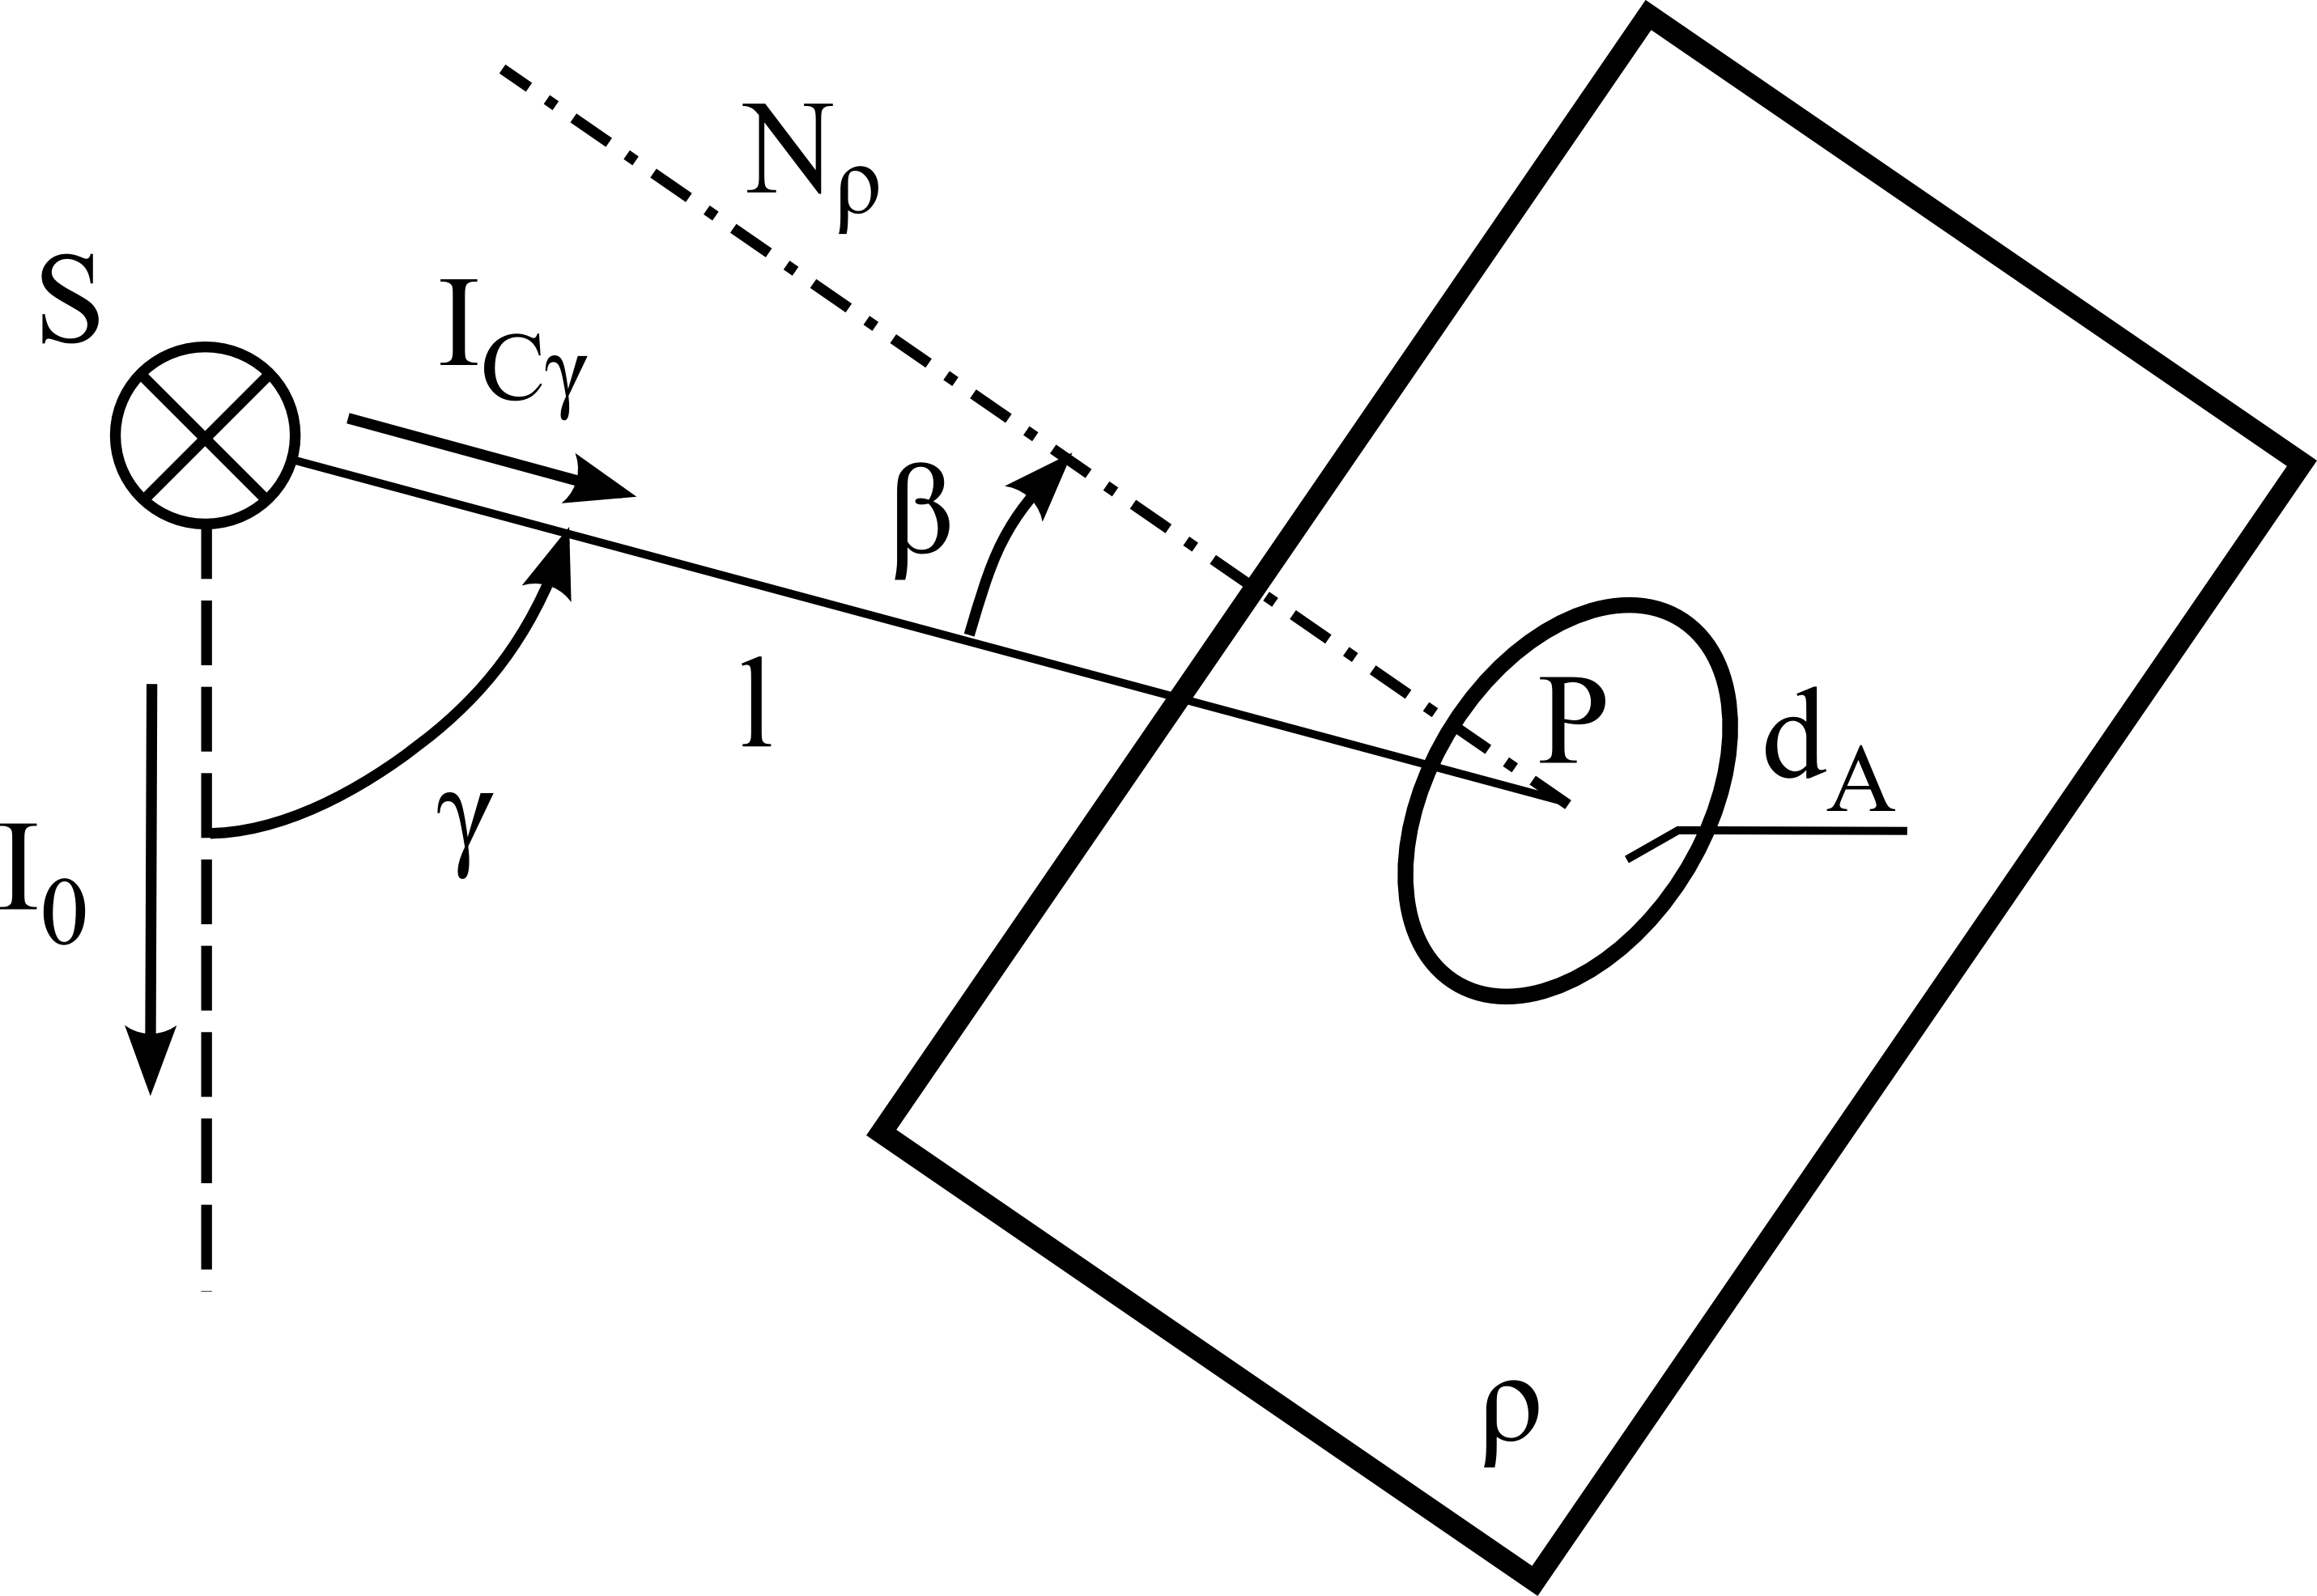
\includegraphics[width=160pt]{315_osvetlenost_bodovym_zdrojem_2}
  \caption{Light source $S$ illuminates point P of plane $\rho$.}
  \label{fig:osv}
\end{figure}

Luminous intensity curves (Equation~\ref{eq:illSum}) can be found in Eulumdat files of luminaires to enable light scene calculations. Most Eulumdat files of indoor luminaires use the $C-\gamma$ angular coordinate system (Figure~\ref{fig:cgamma}).

\begin{figure}[htb]
  \centering
  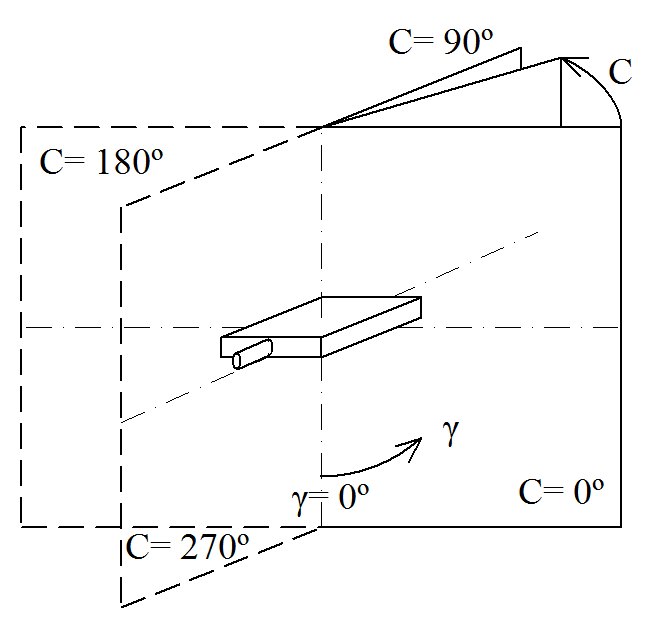
\includegraphics[width=150pt]{Cgama}
  \caption{$C-\gamma$ polar coordinate system with luminaire in center.}
  \label{fig:cgamma}
\end{figure}

To bring simulation results closer to real conditions, interaction of light and surfaces has to be included into calculations the most affecting the light scene in this project being light reflection. In case of the model room light active surfaces are walls, ceiling and floor becoming after light impact secondary light sources. Using the finite element method, surfaces of the model room are divided into smaller facets each becoming a point light source illuminating other facets leading to multiple reflections (Figure~\ref{fig:difRefl}). Each reflection of light a portion of incident luminous flux is consumed by the surface defined by reflectance value $\rho$. After several reflections the reflected luminous flux becomes negligible.

\begin{figure}[htb]
  \centering
  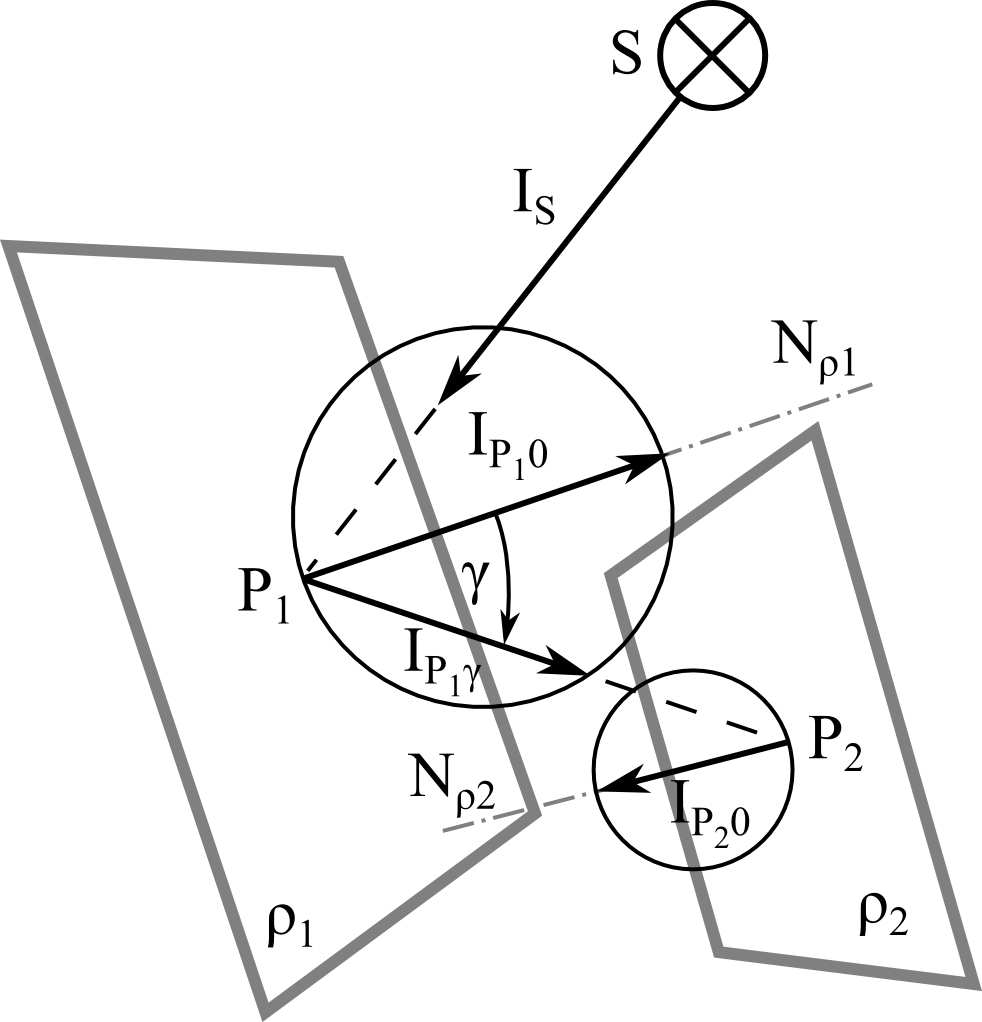
\includegraphics[width=136pt]{diffuseReflection}
  \caption{Multiple reflections between planes $\rho1$ and $\rho2$ with Lambertian reflectance.}
  \label{fig:difRefl}
\end{figure}

Most common indoor wall and ceiling surfaces exhibit near Lambertian (diffuse) reflectance. The spacial luminous intensity distribution of purely Lambertian surfaces is dependent only on luminous intensity $I_{0}$ in direction $\gamma=0^{\circ}$ and on angle~$\gamma$ between the facet's normal~$N_{\rho}$ and the observed direction of the outgoing light ray (Equation~\ref{eq:Igamma}). For simplification reasons all surfaces including the floor of the model room exhibit purely diffuse reflection. Such surfaces become secondary light sources of luminous intensity in direction $\gamma=0^{\circ}$ according to \cite{Habel}:

\begin{equation}
I_{0}=\frac{\rho \cdot E \cdot dA}{\pi} \quad \mathrm{(cd;-,lx,m^{2})}
\label{eq:lumInt}
\end{equation}

where:
\begin{description}
	\item[$I_{0}$] is the luminous intensity of the facet in direction of the facet's normal,
	\item[$\rho$] is the facet's integral reflectance,
	\item[$E$] is the facet's illuminance,
	\item[$dA$] is the facet's area.
\end{description}

After obtaining $I_{0}$, the luminous intensity curve of a facet of Lambertian reflectance will be:

\begin{equation}
I_{\gamma}=I_{0} \cdot \cos(\gamma) \quad \mathrm{(cd;cd,-)}
\label{eq:Igamma}
\end{equation}

where:
\begin{description}
	\item[$I_{\gamma}$] is the luminous intensity in direction $\gamma$,
	\item[$I_{0}$] is the luminous intensity in direction of facet's normal,
	\item[$\gamma$] is the angle between the facet's normal and the line of center points of the source and destination facet.
\end{description}

Calculating resulting luminous intensities of all available facets of the model room is achieved in several steps.

\begin{itemize}
	\item Primary light sources emit light incident on visible facets (direct illumination). Initial illuminance $E_{0\rho}$ of facet $\rho$ is obtained by summing up all partial illuminances from all primary light sources (Equation~\ref{eq:illSum}).
	\item Facets become secondary light sources. Their spacial luminous intensity distributions can be obtained from Equation~\ref{eq:lumInt} and \ref{eq:Igamma} using initial illuminance $E_{0}$. Facet's~$\rho$ illuminance~$E_{1\rho}$ is obtained using Equation~\ref{eq:illSum} and all visible facets as light sources.
	\item 
\end{itemize}

First of all primary light sources emit light incident on those facets. Using Equation~\ref{eq:illSum} facets' illuminances can be calculated. 